\documentclass{beamer}
\usetheme{Szeged}
\usecolortheme{beaver}
\setbeamercovered{transparent}
%%Beamer

%%Packages
\usepackage{amsmath,amsthm,amssymb}
\usepackage{mathrsfs,MnSymbol}
\usepackage{textcomp}
\usepackage{graphicx}
\usepackage{verbatim}
%\usepackage[pdftex,bookmarks=true]{hyperref}
\usepackage{hyperref}
\usepackage{ulem}
%\usepackage{CJK} 

%%TikZ
\usepackage{tikz}
\usetikzlibrary{positioning}
\usetikzlibrary{arrows}
%\usetikzlibrary{bending} % for TikZ 3.0.0
\tikzset{
every picture/.style=thick,
bluenode/.style={circle, draw=black, fill=blue!40, very thick, minimum size=6mm},
whitenode/.style={circle, draw=black, fill=black!10, very thick, minimum size=6mm},
squarednode/.style={rectangle, draw=red!60, fill=red!5, very thick, minimum size=5mm},
every loop/.style={min distance=8mm} %% Default loop has arrow.
}

\newenvironment{drawing}{\begin{center}\begin{tikzpicture}}{\end{tikzpicture}\end{center}}

%%%COLORS%%%
\usepackage{color}
%\definecolor{red}{rgb}{1,0,0}
%\definecolor{blue}{rgb}{0,0,1}
\definecolor{green}{rgb}{0,0.5,0}
\definecolor{lblue}{cmyk}{0.2,0,0,0}
\definecolor{lpurple}{rgb}{.75,.5,.75}
\definecolor{lred}{rgb}{.75,.5,.5}
\definecolor{Tortuga}{rgb}{0.3,0.4,0.1}
%\def\red{\color{red}}
\def\lblue{\color{lblue}}
\def\white{\color{white}}
\usepackage{harpoon}
\def\cellblue{\cellcolor{lblue}}

%%%COLOR TABLE%%%
\usepackage{colortbl} %first try, Feb 2014
\newcolumntype{B}{>{\columncolor{lblue}}c}

%%%MACROS%%%
\def \mr {\operatorname{mr}}
%\def \M {\operatorname{M}}
\def \rank {\operatorname{rank}}
\def \nul {\operatorname{null}}
%\def \erank {\mathrm{erank}}
%\def \tri {\mathrm{tri}}
\def \R {\mathbb{R}}
\def \G {\mathcal{G}}
\def \I {\mathcal{I}}
\def \S {\mathcal{S}}
\def \P {\mathcal{P}}
\def \mt {^{\top}}

\def \wh#1{\widehat{#1}}
\def \GCC#1{#1(G)+#1(\overline{G})\geq n-2}
%\newcommand \wh[1] {\widehat{#1}}

\def \mtx#1{\begin{pmatrix}#1\end{pmatrix}}

%lazy commands
\def \Gll {\widehat{G}_{\ell\ell}}
\def \Hll {\widehat{H}_{\ell\ell}}
\def \GI {\widehat{G}_I}
\def \AE{\mathcal{AE}}
\def \ZE{\mathcal{ZE}}
\def \DE{\mathcal{DE}}
\def \AT{\mathcal{AT}}
\def \ZT{\mathcal{ZT}}
\def \DT{\mathcal{DT}}
\def \mfkG{\mathfrak{G}}
\def \mfkH{\mathfrak{H}}
\def \Zoc{Z_{oc}}
\def \Zhat{\widehat{Z}}
\def \Zochat{\widehat{Z}_{oc}}
\def \blue{{\color{blue} blue}}
\def \white{{\color{gray} white}}
\def \loC{\mathfrak{C}_{2k+1}^0}
\def \Fchar{\operatorname{char}}
\def \Gbar{\overline{G}}
\def \dunion{\mathbin{\dot{\bigcup}}}

\begin{document}

\title[Params Related To The Min Rank Problem \hspace{7em} \insertframenumber/\inserttotalframenumber]{Parameters related to the minimum rank problem}
\author[Jephian C.-H. Lin]{Jephian C.-H. Lin}
\institute[Department of Mathematics, Iowa State University]{
  Department of Mathematics, Iowa State University}
\date[Dec 2, 2014]{Dec 2, 2014\\
Preliminary Exam}

%%%%%%%%%%%%%%%

\begin{frame}
\titlepage
\end{frame}

%%%%%%%

\begin{frame}
\frametitle{Minimum rank problem}
\begin{center}
\begin{tikzpicture}
\draw[black!0] (-5,-2) grid (5,3);
\node[whitenode] (P3) at (-3,3) {2};
\node[whitenode] (P3l) [left= of P3] {1};
\node[whitenode] (P3r) [right= of P3] {3};
\draw (P3l) -- (P3);
\draw (P3) -- (P3r);
\node (pattern) [below= 0 of P3] {$\begin{bmatrix} ? & * & 0 \\ * & ? & * \\ 0 & * & ? \end{bmatrix}$};
\only<2->{\node (question) [right=of pattern, align=center] {\alert{Real, Symmetric}\\What is the smallest possible rank?};}
\only<3-7>{\node (matrix) [below= of pattern] {$\begin{bmatrix} \only<3-5>{1}\only<6-7>{\alert{0}} & 1 & 0 \\ 1 & \only<3-5>{1}\only<6-7>{\alert{0}} & 1 \\ 0 & 1 & \only<3-5>{1}\only<6-7>{\alert{0}} \end{bmatrix}$};
\draw[-triangle 45] (pattern.south) -- (matrix.north);
\node (markl) [right] at (matrix.east) {};
\node (markr) [right=4 of markl] {};}
\only<4>{\draw[-triangle 45] (markl) -- (markr) node[above,  midway]{rank};
\node [right] at (markr.east) {3};}
\only<5>{\draw[-triangle 45] (markl) -- (markr) node[above,  midway]{spectrum};
\node [right] at (markr.east) {$1$, $1\pm\sqrt{2}$};}
\only<7>{\draw[-triangle 45] (markl) -- (markr) node[above,  midway]{rank};
\node [right] at (markr.east) {\alert{2}};}

\end{tikzpicture}
\end{center}
\end{frame}

%%%%%%%

\begin{frame}
\frametitle{Minimum rank problem}
\begin{itemize}
\item Let $G$ be a simple graph. 
\item Denote $\mathcal{S}^F(G)$ as the family of \alert{symmetric} matrices over the field $F$ whose $i,j$-entry, \alert{$i\neq j$}, is nonzero if $i\sim j$ and zero otherwise. (Diagonal entries are free.)
\item The \alert{minimum rank} of $G$ is defined as 
\[\mr^F(G)=\min\{\rank(A):A\in \mathcal{S}^F(G)\}.\]
The \alert{maximum nullity} is 
\[M^F(G)=\max\{\nul(A):A\in \mathcal{S}^F(G)\}.\]
\item $M^F(G)+\mr^F(G)=|V(G)|$ for any $G$ and $F$. 
\end{itemize}
\end{frame}

%%%%%%%

\begin{frame}
\frametitle{Example: Paths $P_n$}
\begin{columns}
\column{0.5\textwidth}
\begin{drawing}
\node (1) [whitenode] at (-1.5,1.5) {};
\node (2) [whitenode] at (-0.5,0.5) {};
\node (4) [whitenode] at (1,-1) {};
\draw (1) -- (2) -- (-0.1,0.1);
\draw [dotted] (0.1,-0.1) -- (0.4,-0.4);
\draw (0.6,-0.6) -- (4);
\end{drawing}
\column{0.5\textwidth}
\[
\begin{bmatrix}
    -1              & 1               & 0      & \cdots          & 0      \\
    {\color{red} 1} & -2              & 1      & ~               & \vdots \\
    0               & {\color{red} 1} & \ddots & \ddots          & 0      \\
    \vdots          & ~               & \ddots & -2              & 1      \\
    0               & \cdots          & 0      & {\color{red} 1} & -1     \\
\end{bmatrix}
\]
\end{columns}
\begin{center}
$M(G)\neq 0$ for all $G$.

$M(G)=1$ iff $G$ is a path.

[Fiedler (1969), Bento and Leal Duarte (2005)\nocite{Fied,BLD}]
\end{center}
\end{frame}

%%%%%%%

\begin{frame}
\frametitle{Example: Complete Graphs $K_n$}
\begin{columns}
\column{0.5\textwidth}
\begin{drawing}
\node (1) [whitenode] at (1,1) {};
\node (2) [whitenode] at (-1,1) {};
\node (3) [whitenode] at (1,-1) {};
\node (4) [whitenode] at (-1,-1) {};
\draw (1) -- (2) -- (3) -- (4) -- (1);
\draw (1) -- (3);
\draw (2) -- (4);
\end{drawing}
\column{0.5\textwidth}
\[
\begin{bmatrix}
1 & 1 & 1 & 1 \\
1 & 1 & 1 & 1 \\
1 & 1 & 1 & 1 \\
1 & 1 & 1 & 1 \\
\end{bmatrix}
\]
\end{columns}
\begin{center}
$M(G)=n$ iff $G=\overline{K_n}$.

$M(G)=n-1$ iff $G=K_n\dunion \overline{K_m}$, $n\geq 2$.
\end{center}
\end{frame}

%%%%%%%

\begin{frame}
\frametitle{Inverse eigenvalue problem}
\begin{center}
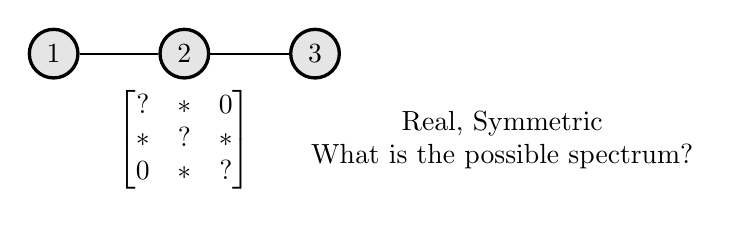
\begin{tikzpicture}
%\draw[black!0] (-5,-2) grid (5,3);
\node[whitenode] (P3) at (-3,3) {2};
\node[whitenode] (P3l) [left= of P3] {1};
\node[whitenode] (P3r) [right= of P3] {3};
\draw (P3l) -- (P3);
\draw (P3) -- (P3r);
\node (pattern) [below= 0 of P3] {$\begin{bmatrix} ? & * & 0 \\ * & ? & * \\ 0 & * & ? \end{bmatrix}$};
\node (question) [right=0.5 of pattern, align=center] {\alert{Real, Symmetric}\\What is the possible \alert{spectrum}?};
\end{tikzpicture}
\end{center}
\begin{itemize}[<+->]
\item We know $\mr(G)=2$ and $M(G)=1$ and Spec$=\{1,1\pm\sqrt{2}\}$ is possible.
\item Can Spec$=\{1,5,5\}$?
\item \alert{No}, for otherwise $\nul(A-5I)=2>M(G)$.
\item Largest possible multiplicity $=M(G)$.
\end{itemize}
\end{frame}

%%%%%%%

\begin{frame}
\frametitle{Inverse eigenvalue problem}
\begin{theorem}[K.~H.~Monfared, B.~L.~Shader 2013\nocite{MS13}]
For a graph $G$ and \alert{distinct} real numbers $\lambda_1,\lambda_2,\ldots,\lambda_n$, there is a matrix $A\in \mathcal{S}^\R(G)$ such that the spectrum of $A$ is $\lambda_1,\lambda_2,\ldots ,\lambda_n$.
\end{theorem}
\vspace{10pt}
\only<2>{For the case multiplicity $\neq 1$, it is still unknown, but the minimum rank problem provides a restriction.}
\end{frame}

%%%%%%%

\begin{frame}
\frametitle{The landscape of minimum rank problems}
\begin{center}
\begin{tikzpicture}[node distance=0.5 and 0.5]
%Nodes
\node (MG) {$M(G)$};
\onslide<1>{\node (Zhat) [above= of MG] {$\Zhat(G)$};}
\node (ZG) [above= of Zhat] {$Z(G)$};
\onslide<1>{\node (MfkG) [below right= 0 and 0.7 of MG] {$M(\mfkG)$};}
\onslide<1>{\node (ZfkG) [above=of MfkG] {$Z(\mfkG)$};}
\onslide<1>{\node (xi) [below= of MG] {$\xi(G)$};}
\node (mu) [below right= of xi] {$\mu(G)$};
\node (Mp) [below left = of MG] {$M_+(G)$};
\onslide<1>{\node (nu) [below = of Mp] {$\nu(G)$};}
\onslide<1>{\node (delta) [below left = 0 and 0.7 of nu] {$\delta(G)$};}
 
%Lines
\onslide<1>{\draw (MG.north) -- (Zhat.south);}
\onslide<1>{\draw (Zhat.north) -- (ZG.south);}
\onslide<1>{\draw (MfkG.north) -- (ZfkG.south);}
\onslide<1>{\draw (ZG.south east) -- (ZfkG.north);}
\draw (MG.south east) -- (mu.north);
\onslide<1>{\draw (MG.south) -- (xi.north);}
\onslide<1>{\draw (xi.south east) -- (mu.north west);}
\onslide<1>{\draw (Mp.south) -- (nu.north);}
\onslide<1>{\draw (xi.south west) -- (nu.north east);}
\onslide<1>{\draw[dashed, -triangle 45] (delta.east) -- (nu.west);}
\onslide<1>{\draw[dashed, -triangle 45] (delta.north east) -- (Mp.south west);}
\onslide<1>{\path[dashed, -triangle 45] (delta.north) edge [bend left] (MG.west);}
\onslide<1>{\path[->] (MfkG.west) edge [bend right] node[above=1mm]{$\max$}(MG.east);}
\onslide<1>{\path[->] (ZfkG.west) edge [bend right] node[above=1mm]{$\max$}(Zhat.east);}
\draw (MG.south west) -- (Mp.north east);
\only<2->{\draw (MG.north) -- (ZG.south);}

\only<2>{
\node [above left= 0 of MG] {maximum nullity};
}
\only<2>{
\node [right=0 of ZG, align=left] {zero forcing number};
}
\only<2>{
\node [left=0 of Mp,align=left] {psd maximum nullity};
}
\only<2>{
\node [left=0 of mu] {Colin de Verdi\`ere parameter};
}

\end{tikzpicture}
\end{center}
\end{frame}

%%%%%%%

\begin{frame}
\frametitle{Zero forcing number}

\begin{itemize}
\item A \alert{zero forcing game} on a simple graph $G$ starts by setting a set $B\subseteq V(G)$ of vertices \blue{} and the others \white{}, and then repeatedly applies the \alert{color-change rule (CCR)}:
\begin{itemize}
\item if $y\in V(G)$ is the only \white{} neighbor of $x\in V(G)$ and $x$ is blue, then $y$ turns \blue{}.
\end{itemize}
\only<3>{
\item The \alert{final coloring} is the set of blue vertices when no more CCR applies.
\item The initial set $B$ is called a \alert{zero forcing set} if its final coloring is $V(G)$.
\item The \alert{zero forcing number} of $G$, denoted as $Z(G)$, is the minimum cardinality of a zero forcing set on $G$.
}
\end{itemize}

\only<1,2>{
\begin{center}
\begin{tikzpicture}
\node[bluenode] (v1) at (-4,1) {};
\node[bluenode] (v2) at (-4,-1) {};
\node[bluenode] (v3) at (-3,0) {x};
\only<1>{\node[whitenode] (v4) at (-1.4,0) {y};}
\only<2>{\node[bluenode] (v4) at (-1.4,0) {y};}
\draw (v1.south east) -- (v3.north west);
\draw (v2.north east) -- (v3.south west);
\draw (v3.east) -- (v4.west);
\end{tikzpicture}
\end{center}
}

\end{frame}

%%%%%%%

\begin{frame}
\frametitle{Example: $5$-sun $H_5$}
\begin{drawing}[scale=0.9]
\node (1) [whitenode] at (90:3) {1};
\node (2) [whitenode] at (90:1.5) {2};
\node (3) [whitenode] at (162:3) {3};
\node (4) [whitenode] at (162:1.5) {4};
\node (5) [whitenode] at (234:3) {5};
\node (6) [whitenode] at (234:1.5) {6};
\node (7) [whitenode] at (306:3) {7};
\node (8) [whitenode] at (306:1.5) {8};
\node (9) [whitenode] at (18:3) {9};
\node (10) [whitenode] at (18:1.5) {{\footnotesize 10}};

\only<2->{
\node (1) [bluenode] at (90:3) {1};
\node (5) [bluenode] at (234:3) {5};
\node (7) [bluenode] at (306:3) {7};
}
\only<3->{
\node (2) [bluenode] at (90:1.5) {2};
\node (6) [bluenode] at (234:1.5) {6};
\node (8) [bluenode] at (306:1.5) {8};
}
\only<4->{
\node (4) [bluenode] at (162:1.5) {4};
\node (10) [bluenode] at (18:1.5) {{\footnotesize 10}};
}
\only<5->{
\node (3) [bluenode] at (162:3) {3};
\node (9) [bluenode] at (18:3) {9};
}

\draw (1) -- (2);
\draw (3) -- (4);
\draw (5) -- (6);
\draw (7) -- (8);
\draw (9) -- (10);
\draw (2) -- (4);
\draw (4) -- (6);
\draw (6) -- (8);
\draw (8) -- (10);
\draw (10) -- (2);

\only<6->{
\draw [->,red] (1) -- (2);
\draw [->,red] (5) -- (6);
\draw [<-,red] (4) -- (6);
\draw [<-,red] (3) -- (4);
\draw [->,red] (7) -- (8);
\draw [->,red] (8) -- (10);
\draw [<-,red] (9) -- (10);
}

\end{drawing}
\begin{center}
$Z(H_5)=3$.
\end{center}
\end{frame}

%%%%%%%

\begin{frame}
\frametitle{Triangle number}
\begin{itemize}
\item Let $Q$ be a pattern (a matrix with entries $\in\{0, * , ?\}$).
\item An upper triangular subpattern is a square submatrix of $Q$ such that the lower part is all \alert{$0$}, diagonals are \alert{ * }.
\item The \alert{triangle number} of $Q$, denoted as $\text{tri}(Q)$, is the largest size of an upper triangular subpattern that can be found in $Q$ through row/column permutations.
\end{itemize}

\[
\begin{bmatrix}
    * & 0 & 0 \\
    ? & \alert{*} & \alert{?} \\
    0 & \alert{0} & \alert{*} \\ 
\end{bmatrix}
\longrightarrow 
\begin{bmatrix}
    ? & \alert{*} & \alert{?} \\
    * & 0 & 0 \\
    0 & \alert{0} & \alert{*} \\
\end{bmatrix}
\longrightarrow 
\begin{bmatrix}
    \alert{*} & ? & ? \\
    0 & \alert{*} & 0 \\
    0 & 0 & \alert{*} \\
\end{bmatrix}
\]
\begin{itemize}
\item If $Q$ is the pattern of a graph $G$, then $\mr(G)\geq \text{tri}(Q)$ and $M(G)\leq n-\text{tri}(Q)$.
\end{itemize}
\end{frame}

%%%%%%%

\begin{frame}
\frametitle{Triangle number of $H_5$?}
\only<1>{
The pattern $Q$ below is the pattern for $H_5$. What is $\text{tri}(Q)$?
\[
\begin{bmatrix}
    ? & * & 0 & 0 & 0 & 0 & 0 & 0 & 0 & 0 \\
    * & ? & 0 & * & 0 & 0 & 0 & 0 & 0 & * \\
    0 & 0 & ? & * & 0 & 0 & 0 & 0 & 0 & 0 \\
    0 & * & * & ? & 0 & * & 0 & 0 & 0 & 0 \\
    0 & 0 & 0 & 0 & ? & * & 0 & 0 & 0 & 0 \\
    0 & 0 & 0 & * & * & ? & 0 & * & 0 & 0 \\
    0 & 0 & 0 & 0 & 0 & 0 & ? & * & 0 & 0 \\
    0 & 0 & 0 & 0 & 0 & * & * & ? & 0 & * \\
    0 & 0 & 0 & 0 & 0 & 0 & 0 & 0 & ? & * \\
    0 & * & 0 & 0 & 0 & 0 & 0 & * & * & ? \\
\end{bmatrix}
\]
}
\only<2>{

\begin{drawing}[scale=0.9]
\node (1) [bluenode] at (90:3) {1};
\node (2) [whitenode] at (90:1.5) {2};
\node (3) [whitenode] at (162:3) {3};
\node (4) [whitenode] at (162:1.5) {4};
\node (5) [bluenode] at (234:3) {5};
\node (6) [whitenode] at (234:1.5) {6};
\node (7) [bluenode] at (306:3) {7};
\node (8) [whitenode] at (306:1.5) {8};
\node (9) [whitenode] at (18:3) {9};
\node (10) [whitenode] at (18:1.5) {{\footnotesize 10}};

\node [left= of 3] {$
\begin{array}{c}
1\rightarrow 2\\
5\rightarrow 6\\
7\rightarrow 8\\
6\rightarrow 4\\
8\rightarrow 10\\
4\rightarrow 3\\
10\rightarrow 9\\
\end{array}
$};

\draw (1) -- (2);
\draw (3) -- (4);
\draw (5) -- (6);
\draw (7) -- (8);
\draw (9) -- (10);
\draw (2) -- (4);
\draw (4) -- (6);
\draw (6) -- (8);
\draw (8) -- (10);
\draw (10) -- (2);

\draw [->,red] (1) -- (2);
\draw [->,red] (5) -- (6);
\draw [<-,red] (4) -- (6);
\draw [<-,red] (3) -- (4);
\draw [->,red] (7) -- (8);
\draw [->,red] (8) -- (10);
\draw [<-,red] (9) -- (10);
\end{drawing}
}
\only<3>{
$\text{tri}(Q)=7$ and $Z(H_5)=3$.
\[
\begin{array}{cc}
~ & \begin{array}{cccccccccc} 1&5&7&6&8&4&10&2&3&9\end{array} \\
\begin{array}{c} 2\\6\\8\\4\\10\\3\\9\\1\\5\\7\\\end{array} & 
\begin{bmatrix}
 {\color{red} *} & 0 & 0 & 0 & 0 & * & *  & ? & 0 & 0 \\
 0 & {\color{red} *} & 0 & ? & * & * & 0  & 0 & 0 & 0 \\
 0 & 0 & {\color{red} *} & * & ? & 0 & *  & 0 & 0 & 0 \\
 0 & 0 & 0 & {\color{red} *} & 0 & ? & 0  & * & * & 0 \\
 0 & 0 & 0 & 0 & {\color{red} *} & 0 & ?  & * & 0 & * \\
 0 & 0 & 0 & 0 & 0 & {\color{red} *} & 0  & 0 & ? & 0 \\
 0 & 0 & 0 & 0 & 0 & 0 & {\color{red} *}  & 0 & 0 & ? \\
 ? & 0 & 0 & 0 & 0 & 0 & 0  & * & 0 & 0 \\
 0 & ? & 0 & * & 0 & 0 & 0  & 0 & 0 & 0 \\
 0 & 0 & ? & 0 & * & 0 & 0  & 0 & 0 & 0 \\
\end{bmatrix}
\end{array}
\]
}
\end{frame}

%%%%%%%

%\begin{frame}
%\frametitle{Let's try!}
%\href{http://bit.ly/1vwYZS0}{http://bit.ly/1vwYZS0}
%\end{frame}

%%%%%%%

\begin{frame}
\frametitle{Zero forcing vs Triangle}
\begin{itemize}
\item Number of \alert{forces} $x_i\rightarrow y_i$ $=$ \alert{size} of triangle.
\item $Z(G)=n-\text{tri}(Q)$, where $Q$ is the pattern of $G$.
\item $M^F(G)\leq Z(G)$, for any simple graph $G$, any field $F$ \nocite{AIM}[AIM Group 2007].
\item It doesn't matter if $\mathcal{S}^F(G)$ is defined to be symmetric or not.
\item $M(G)=Z(G)$ when $|V(G)|\leq 7$ or $G$ is a tree, a cycle, a complete bipartite graph, ...
\item $Z(H_5)=3$ but $M(H_5)=2$.
\end{itemize}
\end{frame}

%%%%%%%



\begin{frame}
\frametitle{The landscape of minimum rank problems}
\begin{center}
\begin{tikzpicture}[node distance=0.5 and 0.5]
%Nodes
\node (MG) {$M(G)$};
\onslide<1>{\node (Zhat) [above= of MG] {$\Zhat(G)$};}
\node (ZG) [above= of Zhat] {$Z(G)$};
\onslide<1>{\node (MfkG) [below right= 0 and 0.7 of MG] {$M(\mfkG)$};}
\onslide<1>{\node (ZfkG) [above=of MfkG] {$Z(\mfkG)$};}
\onslide<1>{\node (xi) [below= of MG] {$\xi(G)$};}
\node (mu) [below right= of xi] {$\mu(G)$};
\node (Mp) [below left = of MG] {$M_+(G)$};
\onslide<1>{\node (nu) [below = of Mp] {$\nu(G)$};}
\onslide<1>{\node (delta) [below left = 0 and 0.7 of nu] {$\delta(G)$};}
 
%Lines
\onslide<1>{\draw (MG.north) -- (Zhat.south);}
\onslide<1>{\draw (Zhat.north) -- (ZG.south);}
\onslide<1>{\draw (MfkG.north) -- (ZfkG.south);}
\onslide<1>{\draw (ZG.south east) -- (ZfkG.north);}
\draw (MG.south east) -- (mu.north);
\onslide<1>{\draw (MG.south) -- (xi.north);}
\onslide<1>{\draw (xi.south east) -- (mu.north west);}
\onslide<1>{\draw (Mp.south) -- (nu.north);}
\onslide<1>{\draw (xi.south west) -- (nu.north east);}
\onslide<1>{\draw[dashed, -triangle 45] (delta.east) -- (nu.west);}
\onslide<1>{\draw[dashed, -triangle 45] (delta.north east) -- (Mp.south west);}
\onslide<1>{\path[dashed, -triangle 45] (delta.north) edge [bend left] (MG.west);}
\onslide<1>{\path[->] (MfkG.west) edge [bend right] node[above=1mm]{$\max$}(MG.east);}
\onslide<1>{\path[->] (ZfkG.west) edge [bend right] node[above=1mm]{$\max$}(Zhat.east);}
\draw (MG.south west) -- (Mp.north east);
\only<2->{\draw (MG.north) -- (ZG.south);}

%\only<2>{
%\node [above left= 0 of MG] {maximum nullity};
%}
%\only<2,3>{
%\node [right=0 of ZG, align=left] {zero forcing number};
%}
\only<2>{
\node [left=0 of Mp,align=left] {psd maximum nullity};
}
%\only<2,5>{
%\node [left=0 of mu] {Colin de Verdi\`ere parameter};
%}

%\only<3>{
%\node [left= 1 of ZG, align=left] {triangle number\\fast mixed search};
%}

\only<2>{
\node [left= 1 of ZG, align=left] {orthogonal representations\\
Maehara Conjecture: $\delta(G)\leq M_+(G)$};
}

%\only<5>{
%\node [left= 1 of ZG, align=left] {$\mu(G)\leq 3$ iff $G$ planar\\Conjecture: $\mu(G)+1\geq \chi(G)$};
%}

\end{tikzpicture}
\end{center}
\end{frame}

%%%%%%%

\begin{frame}
\frametitle{PSD maximum nullity}
\begin{itemize}
\item Denote $\mathcal{S}^\mathbb{F}(G)$ as the family of \alert{symmetric} matrices over $\mathbb{F}$ whose $i,j$-entry, \alert{$i\neq j$}, is nonzero if $i\sim j$ and zero otherwise. (Diagonal entries are free.)
\item $\mathbb{F}=\mathbb{R}$, or $\mathbb{C}$.
\item $\mr_+^\mathbb{F}(G)=\min\{\rank(A):A\in \mathcal{S}^\mathbb{F}(G),~A\text{ is \alert{psd}}\}$.
\item $M_+^\mathbb{F}(G)=\max\{\nul(A):A\in \mathcal{S}^\mathbb{F}(G),~A\text{ is \alert{psd}}\}$.
\end{itemize}

\end{frame}

%%%%%%%

\begin{frame}
\frametitle{PSD Decomposition}
\begin{itemize}
\item Let $A$ be an $n\times n$ (symmetric) psd matrix with $\rank(A)={\color{blue} r}$. 
\item Then 
%\[A=U^*DU=U^*\sqrt{D}\sqrt{D}U=S^*S,\]
%where $S$ can be reduced to a ${\color{red} r}\times n$ matrix.
\[
S^*S=
\begin{bmatrix}
- & v_1^* & - \\
- & v_2^* & - \\
 ~  & \vdots & ~ \\
- & v_n^* & -\\
\end{bmatrix}
\begin{bmatrix}
| & | & ~ & | \\
v_1 & v_2 & \cdots & v_n \\
| & | & ~ & | \\
\end{bmatrix}
=[\langle v_i, v_j \rangle],
\]
where $v_i\in \mathbb{F}^{\color{blue} r}$.
\end{itemize}
\end{frame}

%%%%%%%

\begin{frame}
\frametitle{Orthogonal representation (faithful)}
\begin{itemize}
\item 
\[
S^*S=
\begin{bmatrix}
- & v_1^* & - \\
- & v_2^* & - \\
 ~  & \vdots & ~ \\
- & v_n^* & -\\
\end{bmatrix}
\begin{bmatrix}
| & | & ~ & | \\
v_1 & v_2 & \cdots & v_n \\
| & | & ~ & | \\
\end{bmatrix}
=[\langle v_i, v_j \rangle],
\]
where $v_i\in \mathbb{F}^{\color{blue} r}$.
\item A (faithful) \alert{orthogonal representation} is a function:
\[
\begin{array}{ccc}
V(G) & \longrightarrow & \mathbb{F}^{\color{red} d} \\
i & \longmapsto & v_i 
\end{array}
\text{ such that }
\langle v_i,v_j\rangle \left\{\begin{array}{ll} \neq 0 & \text{if } i\sim j \\ =0 & \text{if } i\nsim j. \end{array}\right.
\]
\item For a given graph $G$, $\min {\color{blue} r} = \min {\color{red} d}$, so $M_+(G)= n-  \min {\color{red} d}$.
\end{itemize}

\end{frame}

%%%%%%%

\begin{frame}
\frametitle{delta conjecture}
\begin{center}
\begin{tikzpicture}[node distance=0.5 and 0.5]
%Nodes
\node (MG) {$M(G)$};
\onslide<1>{\node (Zhat) [above= of MG] {$\Zhat(G)$};}
\node (ZG) [above= of Zhat] {$Z(G)$};
\onslide<1>{\node (MfkG) [below right= 0 and 0.7 of MG] {$M(\mfkG)$};}
\onslide<1>{\node (ZfkG) [above=of MfkG] {$Z(\mfkG)$};}
\onslide<1>{\node (xi) [below= of MG] {$\xi(G)$};}
\node (mu) [below right= of xi] {$\mu(G)$};
\node (Mp) [below left = of MG] {$M_+(G)$};
\onslide<1,5->{\node (nu) [below = of Mp] {$\nu(G)$};}
\onslide<1,3->{\node (delta) [below left = 0 and 0.7 of nu] {$\delta(G)$};}
 
%Lines
\onslide<1>{\draw (MG.north) -- (Zhat.south);}
\onslide<1>{\draw (Zhat.north) -- (ZG.south);}
\onslide<1>{\draw (MfkG.north) -- (ZfkG.south);}
\onslide<1>{\draw (ZG.south east) -- (ZfkG.north);}
\draw (MG.south east) -- (mu.north);
\onslide<1>{\draw (MG.south) -- (xi.north);}
\onslide<1>{\draw (xi.south east) -- (mu.north west);}
\onslide<1,5->{\draw (Mp.south) -- (nu.north);}
\onslide<1>{\draw (xi.south west) -- (nu.north east);}
\onslide<1>{\draw[dashed, -triangle 45] (delta.east) -- (nu.west);}
\only<7->{\draw[densely dotted, -triangle 45,] (delta.east) -- (nu.west);}
\onslide<1,3->{\draw[dashed, -triangle 45] (delta.north east) -- (Mp.south west);}
\onslide<1,6->{\path[dashed, -triangle 45] (delta.north) edge [bend left] (MG.west);}
\onslide<1>{\path[->] (MfkG.west) edge [bend right] node[above=1mm]{$\max$}(MG.east);}
\onslide<1>{\path[->] (ZfkG.west) edge [bend right] node[above=1mm]{$\max$}(Zhat.east);}
\draw (MG.south west) -- (Mp.north east);
\only<2->{\draw (MG.north) -- (ZG.south);}

\only<2->{
\node [right=0 of Mp, blue!60] {Lov\'asz 1979};
}

\only<3->{
\node [below=0 of Mp, blue!70] {~~~~~~~~~Maehara 1987};
}

\only<4->{
\node (kappa) [left= of delta] {$\kappa(G)$};
\path [-triangle 45] (kappa.east) edge (delta.west);
\path [-triangle 45] (kappa.north) edge [bend left] node [left, blue!80] {Lov\'asz et al. 1989} (Mp.west);
%\node [above=0 of kappa, blue!80] {Lov\'asz et al. 1989~~~~~~~~~~};
}

\only<5->{
%\node [above=0 of kappa, blue!85] {van der Holst~2002~~~~~~~~~};
\path [-triangle 45] (kappa.north) edge [bend left] node [left, blue!85, align=center] {van der Holst~~~~~~~\\2002~~~~~~} (nu.west);
}

\only<6->{
\node [above left=0.2 of Mp, blue!90] {Berman et al.~2008};
}

\only<7->{
\node [below=0 of nu, blue!100] {~~~~~T.~Hall~2011+};

}


\end{tikzpicture}
\end{center}
\nocite{Ortho,OrthoC,delta,Hdelta,vdH02}
\end{frame}

%%%%%%%

\begin{frame}
\frametitle{What is $\nu$?}
\begin{itemize}
\item We say a matrix $A$ satisfies \alert{strong Arnol'd Hypothesis} (SAH) if there is \alert{no} nonzero symmetric matrix $X$ satisfying 
\[\left\{\begin{array}{l}I\circ X=O\\A\circ X=O\\ AX=O\\ \end{array}\right.,\]
where $\circ$ is the Hadamard (entrywise) product.
\item $\nu(G)=\max\{\nul(A):A\in\mathcal{S}^{\color{red} \mathbb{R}}(G),~A\text{ is psd},\text{ {\color{red} SAH}}\}$
\item Colin de Verdi\`ere (1998)\nocite{CdV2,HLS} proved  that if $H$ is a minor of $G$, then $\nu(H)\leq \nu(G)$.
\end{itemize}
\end{frame}

%%%%%%%

\begin{frame}
\frametitle{Colin de Verdi\`ere type parameters}
\begin{center}
\begin{tikzpicture}[node distance=0.5 and 0.5]
%Nodes
\node (MG) {$M(G)$};
\onslide<1>{
\node (Zhat) [above= of MG] {$\Zhat(G)$};
}
\node (ZG) [above= of Zhat] {$Z(G)$};
\onslide<1>{
\node (MfkG) [below right= 0 and 0.7 of MG] {$M(\mfkG)$};
\node (ZfkG) [above=of MfkG] {$Z(\mfkG)$};
}
\node (xi) [below= of MG] {$\xi(G)$};
\node (mu) [below right= of xi] {$\mu(G)$};
\node (Mp) [below left = of MG] {$M_+(G)$};
\node (nu) [below = of Mp] {$\nu(G)$};
\onslide<1>{
\node (delta) [below left = 0 and 0.7 of nu] {$\delta(G)$};
}
 
%Lines
\onslide<1>{
\draw (MG.north) -- (Zhat.south);
\draw (Zhat.north) -- (ZG.south);
\draw (MfkG.north) -- (ZfkG.south);
\draw (ZG.south east) -- (ZfkG.north);
}
\draw (MG.south east) -- (mu.north);
\draw (MG.south) -- (xi.north);
\draw (xi.south east) -- (mu.north west);
\draw (Mp.south) -- (nu.north);
\draw (xi.south west) -- (nu.north east);
\onslide<1>{
\draw[dashed, -triangle 45] (delta.east) -- (nu.west);
\path[->] (MfkG.west) edge [bend right] node[above=1mm]{$\max$}(MG.east);
\path[->] (ZfkG.west) edge [bend right] node[above=1mm]{$\max$}(Zhat.east);
}
\draw (MG.south west) -- (Mp.north east);
\only<2>{
\draw (MG.north) -- (ZG.south);
}

\only<2->{
\node [left = 0 of MG] {{\color{green} $\mathcal{S}^F(G)$}};
\node [left = 0 of Mp] {{\color{green} $\mathcal{S}^F(G)$},{\color{blue} psd}};
\node [left = 0 of nu] {{\color{green} $\mathcal{S}^F(G)$},{\color{blue} psd},{\color{red} SAH}};
\node [below = 0 of xi, align=center] {{\color{green} $\mathcal{S}^F(G)$}\\{\color{red} SAH}};
\node [right = 0 of mu, align=left] {{\color{green} gen Laplacian}\\{\color{blue} 1 neg eigen}\\{\color{red} SAH}};
}
\end{tikzpicture}
\end{center}
\end{frame}

%%%%%%%

\begin{frame}
\frametitle{Colin de Verdi\`ere parameter $\mu$}
\begin{itemize}
\item $\mu(G)$ is defined as the maximum nullity among matrices $M$ with the following properties:
\begin{itemize}
\item {\color{green} Generalized Laplacian}: $M_{ij}\left\{\begin{array}{lll} < 0 &\text{if}& i\sim j,i\neq j\\ =0 & \text{if} & i\nsim j, i\neq j \\ \text{ free} & \text{if} & i=j \end{array}\right.$.
\item $M$ has exactly {\color{blue} one negative eigenvalue}.
\item $M$ satisfies {\color{red} SAH}.
\end{itemize}
\item $\mu(G)$ bridges \alert{algebraic} and \alert{topological} properties of a graph [Colin de Verdi\`ere, Robertson et al., Lov\'asz et al.\nocite{CdV, RST93, LSch98}]:
\begin{itemize}
\item $\mu(G)\leq 1$ iff $G$ is a disjoint union of paths;
\item $\mu(G)\leq 2$ iff $G$ is outerplanar;
\item $\mu(G)\leq 3$ iff $G$ is planar;
\item $\mu(G)\leq 4$ iff $G$ is linklessly embedable.
\end{itemize}
\item Colin de Verdi\`ere\nocite{CdV} conjectured $\chi(G)\leq \mu(G)+1$.
\end{itemize}
\end{frame}

%%%%%%%

\begin{frame}
\frametitle{Graph Complement Conjecture (GCC)}
\begin{itemize}
\item Let $G$ be a simple graph and $\beta(G)$ a parameter of $G$. Then GCC-$\beta$ states that $\beta(G)+\beta(\overline{G})\geq n-2$.
\begin{itemize}
\item Kotlov (1997)\nocite{KLV} conjectured GCC-$\mu$.
\item Brualdi et al.~(2007)\nocite{AIMrpt} conjectured GCC-$M$.
\item Barioli et al.~(2012)\nocite{GCC} conjectured GCC-$M_+$ and GCC-$\nu$.
\item ISU EGR group (2011)\nocite{EGR11} proved GCC-$Z$, GCC-$Z_+$, and GCC-$\text{tw}$.
\end{itemize}
\end{itemize}
\end{frame}

%%%%%%%

\begin{frame}
\frametitle{Graph Complement Conjecture}
\begin{center}
\begin{tikzpicture}[node distance=0.5 and 0.5]
%Nodes
\node (MG) {$M(G)$};
\only<1,2,3,4>{
\node (Zhat) [above= of MG] {$\Zhat(G)$};
\node (ZG) [above= of Zhat] {$Z(G)$};
}
\only<5->{
\node [blue] (Zhat) [above= of MG] {$\Zhat(G)$};
\node [blue] (ZG) [above= of Zhat] {$Z(G)$};
\node [blue] (Zp) [above= of Mp] {$Z_+(G)$};
\node [blue] (tw) [below left= of Zp] {$\text{tw}(G)$};
\draw [-triangle 45] (Zp.north east) -- (Zhat.south west);
\draw [-triangle 45] (tw.north east) -- (Zp.south west);
\draw [-triangle 45] (Mp.north) -- (Zp.south);
}
\onslide<1>{
\node (MfkG) [below right= 0 and 0.7 of MG] {$M(\mfkG)$};
\node (ZfkG) [above=of MfkG] {$Z(\mfkG)$};
}
\node (xi) [below= of MG] {$\xi(G)$};
\node (mu) [below right= of xi] {$\mu(G)$};
\node (Mp) [below left = of MG] {$M_+(G)$};
\node (nu) [below = of Mp] {$\nu(G)$};
\only<1,2>{
\node (delta) [below left = 0 and 0.7 of nu] {$\delta(G)$};
\node (kappa) [left= of delta] {$\kappa(G)$};
}

\only<3>{
\node [red] (delta) [below left = 0 and 0.7 of nu] {$\delta(G)$};
\node [red] (kappa) [left= of delta] {$\kappa(G)$};
}
\only<4->{
\node [red] (delta) [below left = 0 and 0.7 of nu] {$\lceil\delta(G)\rceil$};
\node [red] (kappa) [left= of delta] {$\lceil\kappa(G)\rceil$};
}

 
%Lines
\draw (MG.north) -- (Zhat.south);
\draw (Zhat.north) -- (ZG.south);
\onslide<1>{
\draw (MfkG.north) -- (ZfkG.south);
\draw (ZG.south east) -- (ZfkG.north);
}
\draw (MG.south east) -- (mu.north);
\draw (MG.south) -- (xi.north);
\draw (xi.south east) -- (mu.north west);
\draw (Mp.south) -- (nu.north);
\draw (xi.south west) -- (nu.north east);
\draw[dashed, -triangle 45] (delta.east) -- (nu.west);
\onslide<1>{
\path[->] (MfkG.west) edge [bend right] node[above=1mm]{$\max$}(MG.east);
\path[->] (ZfkG.west) edge [bend right] node[above=1mm]{$\max$}(Zhat.east);
}
\draw (MG.south west) -- (Mp.north east);
\draw [-triangle 45] (kappa.east) -- (delta.west);


\only<2->{
\draw [-triangle 45] (MG.north) -- (Zhat.south);
\draw [-triangle 45] (Zhat.north) -- (ZG.south);
\draw [triangle 45-] (MG.south east) -- (mu.north);
\draw [triangle 45-] (MG.south) -- (xi.north);
\draw [triangle 45-] (xi.south east) -- (mu.north west);
\draw [triangle 45-] (Mp.south) -- (nu.north);
\draw [triangle 45-] (xi.south west) -- (nu.north east);
\draw [dashed, -triangle 45] (delta.east) -- (nu.west);
\draw [triangle 45-] (MG.south west) -- (Mp.north east);
}

\end{tikzpicture}
\end{center}
\nocite{EGR11,NGSurvey}
\end{frame}

%%%%%%%

\begin{frame}
\frametitle{Loop graphs}
\begin{itemize}
\item A \alert{loop graph} $\mathfrak{G}$ is a graph where loops are allowed. (Each vertex has at most one loop.)
\item A \alert{loop configuration} $\mathfrak{G}$ of a simple graph $G$ is a loop graph obtained from $G$ by designating each vertex as having no loop or one loop. (There are $2^n$ possibilities.)
\item $M^F(\mfkG)=\max \left\{\nul(A):A\in\mathcal{S}^F(G), A_{i,i}\Big\{\begin{array}{lll}\neq 0 & \text{if} & i\text{ has a loop;}\\ =0 & \text{if} & i\text{ has no loop}.\end{array}\right\}$.
\item $M^F(G)=\max_\mfkG M^F(\mfkG)$, where $\mfkG$ runs over all loop configurations of $\mfkG$.

\end{itemize}
\end{frame}

%%%%%%%

\begin{frame}
\frametitle{$Z(\mfkG)$ for loop graphs / $\Zhat(G)$ for simple graphs}
\begin{itemize}
\item The \alert{color-change rule} for loop graphs is:
\begin{itemize}
\item if $y\in V(\mfkG)$ is the only \white{} neighbor of $x\in V(\mfkG)$ \sout{and $x$ is \blue{}}, then $y$ turns \blue{}. (\alert{$x=y$ is possible}.)
\end{itemize}
\only<5->{
\item $Z(\mfkG)$ is the smallest cardinality of a zero forcing set on $\mfkG$ \alert{using CCR for loop graphs}.
\item $M^F(\mfkG)\leq Z(\mfkG)$ for all loop graphs $\mfkG$ and fields $F$ [Hogben (2010)\nocite{cancun}].
\item If $\mfkG$ is a loop configuration of $G$, then $Z(\mfkG)\leq Z(G)$.
\item The \alert{enhanced zero forcing number} is defined as $\Zhat(G)=\max_\mfkG Z(\mfkG)$, where $\mfkG$ runs over all loop configurations of $G$.
}
\end{itemize}

\only<1,2,3,4>{
\begin{drawing}
\node[whitenode] (x) at (-1.5,0) {x};
\node[whitenode] (y) at (0,0) {y};
\node[whitenode] (z) at (1.5,0) {z};
\draw (x) -- (y) --(z);
\path [dashed] (x) edge [loop above] ();
\path [dashed] (y) edge [loop above] ();
\path (z) edge [loop above] ();
\only<2->{
\node[bluenode] (y) at (0,0) {y};
}
\only<3->{
\node[bluenode] (z) at (1.5,0) {z};
}
\only<4>{
\node[bluenode] (x) at (-1.5,0) {x};
}
\end{drawing}
}

\end{frame}

%%%%%%%

\begin{frame}
\frametitle{$H_5$ revisited}
\begin{drawing}[scale=0.9]
\node (1) [whitenode] at (90:3) {1};
\node (2) [whitenode] at (90:1.5) {2};
\node (3) [whitenode] at (162:3) {3};
\node (4) [whitenode] at (162:1.5) {4};
\node (5) [whitenode] at (234:3) {5};
\node (6) [whitenode] at (234:1.5) {6};
\node (7) [whitenode] at (306:3) {7};
\node (8) [whitenode] at (306:1.5) {8};
\node (9) [whitenode] at (18:3) {9};
\node (10) [whitenode] at (18:1.5) {{\footnotesize 10}};

\only<2-7>{
\node [right=of 1, align=left] {$1$ has a loop and\\the others are {\color{red} unknown}.};
\path (1) edge [loop left] ();
}
\only<8-12>{
\node [right=of 1, align=left] {$1$ has no loop and\\the others are {\color{red} unknown}.};
\path (1) edge [dashed, loop left] ();
}

\only<2-7>{
\node (3) [bluenode] at (162:3) {3};
\node (5) [bluenode] at (234:3) {5};
}
\only<3-7>{
\node (4) [bluenode] at (162:1.5) {4};
\node (6) [bluenode] at (234:1.5) {6};
}
\only<4-7>{
\node (2) [bluenode] at (90:1.5) {2};
\node (8) [bluenode] at (306:1.5) {8};
}
\only<5-7>{
\node (1) [bluenode] at (90:3) {1};
}
\only<6-7>{
\node (10) [bluenode] at (18:1.5) {{\footnotesize 10}};
}
\only<7>{
\node (7) [bluenode] at (306:3) {7};
\node (9) [bluenode] at (18:3) {9};
}
\only<8-12>{
\node (5) [bluenode] at (234:3) {5};
\node (7) [bluenode] at (306:3) {7};
}
\only<9-12>{
\node (6) [bluenode] at (234:1.5) {6};
\node (8) [bluenode] at (306:1.5) {8};
}
\only<10-12>{
\node (4) [bluenode] at (162:1.5) {4};
\node (10) [bluenode] at (18:1.5) {{\footnotesize 10}};
}
\only<11-12>{
\node (2) [bluenode] at (90:1.5) {2};
}
\only<12>{
\node (1) [bluenode] at (90:3) {1};
\node (3) [bluenode] at (162:3) {3};
\node (9) [bluenode] at (18:3) {9};
}

\draw (1) -- (2);
\draw (3) -- (4);
\draw (5) -- (6);
\draw (7) -- (8);
\draw (9) -- (10);
\draw (2) -- (4);
\draw (4) -- (6);
\draw (6) -- (8);
\draw (8) -- (10);
\draw (10) -- (2);

\end{drawing}
\begin{center}
$\Zhat(H_5)=2$ and $Z(H_5)=3$.
\end{center}
\end{frame}

%%%%%%%

\begin{frame}[fragile]
\frametitle{Sage Data}
\begin{itemize}
\item $M(G)=\Zhat(G)=Z(G)$ if $|V(G)|\leq 7$.
\item For $n=8$, there are $7$ graphs with $\Zhat(G)<Z(G)$.
\item For $n=9$, there are $412$ graphs with $\Zhat(G)<Z(G)$.
\item For $n=10$, there are $18700+$ graphs with $\Zhat(G)<Z(G)$.
\item But $M(K_{3,3,3})=6$ and $Z(G)=\Zhat(G)=7$.
\end{itemize}
\end{frame}

%%%%%%%

\begin{frame}
\frametitle{New parameters $\Zochat(G)$ and $\Zoc(\mfkG)$}
\begin{center}
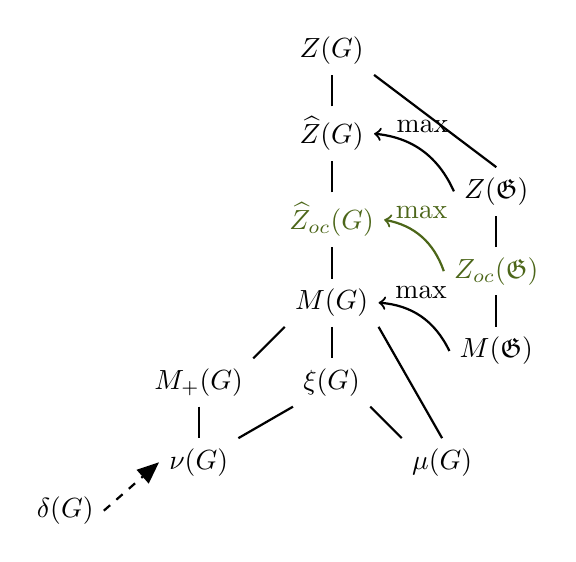
\begin{tikzpicture}[node distance=0.4 and 0.4]
%Nodes
\node (MG) {$M(G)$};
\node [Tortuga] (Zochat) [above= of MG] {$\Zochat(G)$};
\node (Zhat) [above= of Zochat] {$\Zhat(G)$};
\node (ZG) [above= of Zhat] {$Z(G)$};
\node (MfkG) [below right= 0 and 0.9 of MG] {$M(\mfkG)$};
\node [Tortuga] (ZocfkG) [above=of MfkG] {$\Zoc(\mfkG)$};
\node (ZfkG) [above=of ZocfkG] {$Z(\mfkG)$};
\node (xi) [below= of MG] {$\xi(G)$};
\node (mu) [below right= of xi] {$\mu(G)$};
\node (Mp) [below left = of MG] {$M_+(G)$};
\node (nu) [below = of Mp] {$\nu(G)$};
\node (delta) [below left = 0 and 0.7 of nu] {$\delta(G)$};

%Lines
\draw (MG.north) -- (Zochat.south);
\draw (Zochat.north) -- (Zhat.south);
\draw (Zhat.north) -- (ZG.south);
\draw (MfkG.north) -- (ZocfkG.south);
\draw (ZocfkG.north) -- (ZfkG.south);
\draw (ZG.south east) -- (ZfkG.north);
\draw (MG.south east) -- (mu.north);
\draw (MG.south) -- (xi.north);
\draw (xi.south east) -- (mu.north west);
\draw (Mp.south) -- (nu.north);
\draw (xi.south west) -- (nu.north east);
\draw[dashed, -triangle 45] (delta.east) -- (nu.west);
\path[->] (MfkG.west) edge [bend right] node[above=1mm]{$\max$}(MG.east);
\path[->] (ZocfkG.west) edge [Tortuga, bend right] node[above=1mm]{$\max$}(Zochat.east);
\path[->] (ZfkG.west) edge [bend right] node[above=1mm]{$\max$}(Zhat.east);
\draw (MG.south west) -- (Mp.north east);

\end{tikzpicture}
\end{center}
\end{frame}

%%%%%%%

\begin{frame}
\frametitle{Odd cycles}
\begin{itemize}
\item $\Zhat(G)$ shows a bound for $M(\mfkG)$ leads to a bound for $M(G)$; an improvement of bounds for loop graphs leads to an improvement for simple graphs.
\item Let $\loC$ be a \alert{loopless odd cycle}, as a loop graph. Then $M(\loC)=0$ but $Z(\loC)=1$.
\end{itemize}
\begin{columns}
\column{0.5\textwidth}
\begin{drawing}
\node (1) [whitenode] at (90:1) {1};
\node (2) [whitenode] at (162:1) {2};
\node (3) [whitenode] at (234:1) {3};
\node (4) [whitenode] at (306:1) {4};
\node (5) [whitenode] at (18:1) {5};

\draw (1) -- (2) -- (3) -- (4) -- (5) -- (1);
\path [dashed] (1) edge [loop left] ();
\path [dashed] (2) edge [loop left] ();
\path [dashed] (3) edge [loop left] ();
\path [dashed] (4) edge [loop right] ();
\path [dashed] (5) edge [loop right] ();
\end{drawing}
\column{0.5\textwidth}
\[
\det \begin{bmatrix}
    {\color{red} 0}        & e_1    & ~  & ~       & e_{2k+1} \\
    e_1      & {\color{red} 0}       & e_2     & ~       & ~   \\
    ~   & e_2    & \ddots  & \ddots  & ~        \\
    ~        & ~      & \ddots  & ~       & e_{2k}   \\
    e_{2k+1} & ~ & ~       & e_{2k}  & {\color{red} 0}         \\
\end{bmatrix}
\]
\[
=2\prod_{i=1}^{2k+1} e_i
\]
\end{columns}
\end{frame}

%%%%%%%

\begin{frame}
\frametitle{Try to generalize triangle number}
\[
\rank
\begin{bmatrix}
    \only<1>{a_{1,1}}\only<2>{A_{1,1}}\only<3>{A(\mathfrak{C}_5^0)} & ?                                                              & ?                                                              & ? & ? \\
    \only<1>{0}\only<2,3>{O}                                                              & \only<1>{a_{2,2}}\only<2>{A_{2,2}}\only<3>{A(\mathfrak{C}_7^0)} & ?                                                              & ? & ? \\
    \only<1>{0}\only<2,3>{O}                                                                & \only<1>{0}\only<2,3>{O}                                                                & \only<1>{a_{3,3}}\only<2>{A_{3,3}}\only<3>{A(\mathfrak{C}_3^0)} & ? & ? \\
    ?                                                              & ?                                                              & ?                                                              & ? & ? \\
    ?                                                              & ?                                                              & ?                                                              & ? & ? \\
\end{bmatrix}
\geq \only<1>{3}\only<2>{\sum_{i=1}^3\rank(A_{i,i})}\only<3>{5+7+3=15}
\]
\end{frame}

%%%%%%%

\begin{frame}
\frametitle{Odd cycle zero forcing number}

\begin{itemize}
\item The \alert{color-change rule} \alert{CCR-$\Zoc$} for loop graphs is:
\begin{itemize}
\item if $y\in V(\mfkG)$ is the only \white{} neighbor of $x\in V(\mfkG)$ \sout{and $x$ is \blue{}}, then $y$ turns \blue{} (\alert{$x=y$ is possible});
\item if $W$ is the set of \white{} vertices, and $\mfkG[W]$ has a connected component $\mathfrak{C}$ such that $\mathfrak{C}\cong \loC$, then all vertices in $V(\mathfrak{C})$ turn blue.
\end{itemize}
\only<6->{
\item $\Zoc(\mfkG)$ is the smallest cardinality of a zero forcing set on $\mfkG$ \alert{using CCR-$\Zoc$ for loop graphs}.
\item $M^F(\mfkG)\leq \Zoc(\mfkG)$ whenever $\Fchar F\neq 2$ and matrices are symmetric.
\item The \alert{enhanced odd cycle zero forcing number} is defined as $\Zochat(G)=\max_\mfkG \Zoc(\mfkG)$, where $\mfkG$ runs over all loop configurations of $G$.
}
\end{itemize}

\only<1-5>{
\begin{drawing}
\node[whitenode] (v1) at (-4,1) {};
\node[whitenode] (v2) at (-4,-1) {};
\node[whitenode] (v3) at (-3,0) {};
\node[whitenode] (v4) at (-1.4,0) {};
\node[whitenode] (v5) at (0.2,0) {};
\node[whitenode] (v6) at (1.2,1) {};
\node[whitenode] (v7) at (1.2,-1) {};
\draw (v1) -- (v2);
\draw (v1) -- (v3);
\draw (v1) -- (v4);
\draw (v2) -- (v3);
\draw (v2) -- (v4);
\draw (v4) -- (v5);
\draw (v4) -- (v6);
\draw (v4) -- (v7);
\draw (v5) -- (v6);
\draw (v5) -- (v7);
\draw (v6) -- (v7);
\draw (v3.east) -- (v4.west);
\path [dashed] (v1) edge [loop left] ();
\path [dashed] (v2) edge [loop left] ();
\path [dashed] (v3) edge [loop left] ();
\path [dashed] (v4) edge [loop above] ();
\path [dashed] (v5) edge [loop right] ();
\path [dashed] (v6) edge [loop right] ();
\path [dashed] (v7) edge [loop right] ();

\only<1->{\node[bluenode] (v4) at (-1.4,0) {};}
\only<2>{
\node[bluenode] (v1) at (-4,1) {};
\node[bluenode] (v2) at (-4,-1) {};
\node[bluenode] (v3) at (-3,0) {};
\node[bluenode] (v5) at (0.2,0) {};
\node[bluenode] (v6) at (1.2,1) {};
\node[bluenode] (v7) at (1.2,-1) {};
}
\only<3->{
\node[bluenode] (v1) at (-4,1) {};
\node[bluenode] (v6) at (1.2,1) {};
}
\only<4->{
\node[bluenode] (v2) at (-4,-1) {};
\node[bluenode] (v7) at (1.2,-1) {};
}
\only<5->{
\node[bluenode] (v3) at (-3,0) {};
\node[bluenode] (v5) at (0.2,0) {};
}
\end{drawing}
}


\end{frame}

%%%%%%%

\begin{frame}
\frametitle{Example: $K_{3,3,3}$}
\begin{drawing}[scale=0.8]
\node (1) [whitenode] at (130:3) {1};
\node (2) [whitenode] at (150:3) {2};
\node (3) [whitenode] at (170:3) {3};
\node (4) [whitenode] at (250:3) {4};
\node (5) [whitenode] at (270:3) {5};
\node (6) [whitenode] at (290:3) {6};
\node (7) [whitenode] at (10:3) {7};
\node (8) [whitenode] at (30:3) {8};
\node (9) [whitenode] at (50:3) {9};

\only<2,3>{
\node (4) [bluenode] at (250:3) {4};
\node (5) [bluenode] at (270:3) {5};
\node (6) [bluenode] at (290:3) {6};
\node (7) [bluenode] at (10:3) {7};
\node (8) [bluenode] at (30:3) {8};
\node (9) [bluenode] at (50:3) {9};
\path (1) edge [loop left] ();
\path (2) edge [loop left] (); 
\path (3) edge [loop left] (); 
\node [left= of 2, align=center] {1,2,3 have loops\\ others are {\color{red} unknown}};
}
\only<3>{
\node (1) [bluenode] at (130:3) {1};
\node (2) [bluenode] at (150:3) {2};
\node (3) [bluenode] at (170:3) {3};
}
\only<4,5>{
\node (2) [bluenode] at (150:3) {2};
\node (3) [bluenode] at (170:3) {3};
\node (5) [bluenode] at (270:3) {5};
\node (6) [bluenode] at (290:3) {6};
\node (8) [bluenode] at (30:3) {8};
\node (9) [bluenode] at (50:3) {9};
\path (1) edge [dashed, loop left] ();
\path (4) edge [dashed, loop left] (); 
\path (7) edge [dashed, loop right] (); 
\node [left= of 2, align=center] {1,4,7 have no loops\\ others are {\color{red} unknown}};
}
\only<5>{
\node (1) [bluenode] at (130:3) {1};
\node (4) [bluenode] at (250:3) {4};
\node (7) [bluenode] at (10:3) {7};
}

\draw (1) -- (4);
\draw (1) -- (5);
\draw (1) -- (6);
\draw (1) -- (7);
\draw (1) -- (8);
\draw (1) -- (9);
\draw (2) -- (4);
\draw (2) -- (5);
\draw (2) -- (6);
\draw (2) -- (7);
\draw (2) -- (8);
\draw (2) -- (9);
\draw (3) -- (4);
\draw (3) -- (5);
\draw (3) -- (6);
\draw (3) -- (7);
\draw (3) -- (8);
\draw (3) -- (9);
\draw (4) -- (7);
\draw (4) -- (8);
\draw (4) -- (9);
\draw (5) -- (7);
\draw (5) -- (8);
\draw (5) -- (9);
\draw (6) -- (7);
\draw (6) -- (8);
\draw (6) -- (9);

\end{drawing}
\begin{center}
$\Zochat(K_{3,3,3})=6$ and $\Zhat(K_{3,3,3})=Z(K_{3,3,3})=7$.
\end{center}

\end{frame}

%%%%%%%

\begin{frame}
\frametitle{GCC-$\Zochat(G)$}
\begin{center}
\begin{tikzpicture}[node distance=0.4 and 0.4]
%Nodes
\node (MG) {$M(G)$};
\node [blue] (Zochat) [above= of MG] {$\Zochat(G)$};
\node [blue](Zhat) [above= of Zochat] {$\Zhat(G)$};
\node [blue] (ZG) [above= of Zhat] {$Z(G)$};
\node (MfkG) [below right= 0 and 0.9 of MG] {$M(\mfkG)$};
\only<1>{\node [Tortuga] (ZocfkG) [above=of MfkG] {$\Zoc(\mfkG)$};}
\only<2>{\node (ZocfkG) [above=of MfkG] {$\Zoc(\mfkG)$};}
\node (ZfkG) [above=of ZocfkG] {$Z(\mfkG)$};
\node (xi) [below= of MG] {$\xi(G)$};
\node (mu) [below right= of xi] {$\mu(G)$};
\node (Mp) [below left = of MG] {$M_+(G)$};
\node (nu) [below = of Mp] {$\nu(G)$};
\node [red] (delta) [below left = 0 and 0.7 of nu] {$\lceil\delta(G)\rceil$};
\node (Zp) [blue, above = of Mp] {$Z_+(G)$};
\node (tw) [blue, below left= of Zp] {$\text{tw}(G)$};

%Lines
\draw (MG.north) -- (Zochat.south);
\draw (Zochat.north) -- (Zhat.south);
\draw (Zhat.north) -- (ZG.south);
\draw (MfkG.north) -- (ZocfkG.south);
\draw (ZocfkG.north) -- (ZfkG.south);
\draw (ZG.south east) -- (ZfkG.north);
\draw (MG.south east) -- (mu.north);
\draw (MG.south) -- (xi.north);
\draw (xi.south east) -- (mu.north west);
\draw (Mp.south) -- (nu.north);
\draw (xi.south west) -- (nu.north east);
\draw[dashed, -triangle 45] (delta.east) -- (nu.west);
\path[->] (MfkG.west) edge [bend right] node[above=1mm]{$\max$}(MG.east);
\only<1>{\path[->] (ZocfkG.west) edge [Tortuga, bend right] node[above=1mm]{$\max$}(Zochat.east);}
\only<2>{\path[->] (ZocfkG.west) edge [bend right] node[above=1mm]{$\max$}(Zochat.east);}
\path[->] (ZfkG.west) edge [bend right] node[above=1mm]{$\max$}(Zhat.east);
\draw (MG.south west) -- (Mp.north east);
\draw (tw.north east) -- (Zp.south west);
\draw (Zp.north east) -- (Zochat.south west);
\draw (Mp.north) -- (Zp.south);

\node (kappa) [red,left= of delta] {$\lceil\kappa(G)\rceil$};
\draw (kappa.east) -- (delta.west);

\only<2>{
\node (Zmu) [Tortuga, above= of mu] {$Z_\mu$?}; 
\draw [Tortuga] (mu.north) -- (Zmu.south);
}

\end{tikzpicture}
\end{center}
\end{frame}

%%%%%%%

\begin{frame}
\frametitle{Bound $\mu$ above}
\begin{itemize}
\item Recall that $\mu(G)$ is the maximum nullity among matrices $M$ with the following properties:
\begin{itemize}
\item {\color{green} Generalized Laplacian}: $M_{ij}\left\{\begin{array}{lll} < 0 &\text{if}& i\sim j,i\neq j\\ =0 & \text{if} & i\nsim j, i\neq j \\ \text{ free} & \text{if} & i=j \end{array}\right.$.
\item $M$ has exactly {\color{blue} one negative eigenvalue}.
\item $M$ satisfies {\color{red} SAH}.
\end{itemize}
\item Goldberg and Berman (2014)\nocite{GB14} found $Z_\pm$ to bound $M(Q_\pm)$.
\item Butler et al.~(2014)\nocite{Zq} found $Z_q$ to bound $M_q(G)$.
\item So $\mu(G)\leq \min\{Z_\pm(G),Z_1(G)\}$, but can we do better?
\item If such $Z_\mu$ exists, is GCC-$Z_\mu$ true or not?
\end{itemize}
\end{frame}

%%%%%%%

\begin{frame}
\frametitle{Transferring from $\nu$ to $\mu$}
\begin{center}
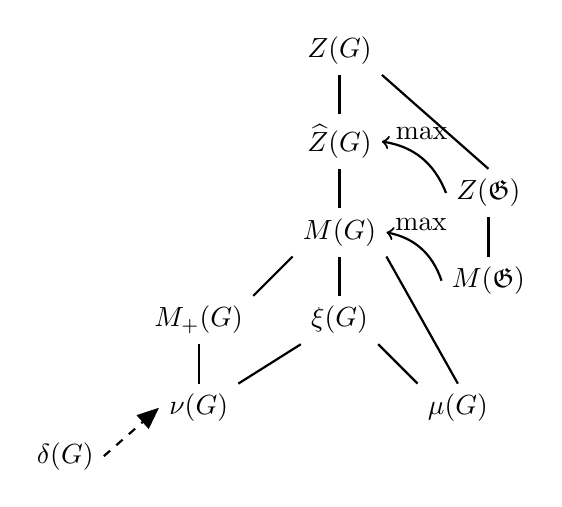
\begin{tikzpicture}[node distance=0.5 and 0.5]
%Nodes
\node (MG) {$M(G)$};
\node (Zhat) [above= of MG] {$\Zhat(G)$};
\node (ZG) [above= of Zhat] {$Z(G)$};
\node (MfkG) [below right= 0 and 0.7 of MG] {$M(\mfkG)$};
\node (ZfkG) [above=of MfkG] {$Z(\mfkG)$};
\node (xi) [below= of MG] {$\xi(G)$};
\node (mu) [below right= of xi] {$\mu(G)$};
\node (Mp) [below left = of MG] {$M_+(G)$};
\node (nu) [below = of Mp] {$\nu(G)$};
\node (delta) [below left = 0 and 0.7 of nu] {$\delta(G)$};

%Lines
\draw (MG.north) -- (Zhat.south);
\draw (Zhat.north) -- (ZG.south);
\draw (MfkG.north) -- (ZfkG.south);
\draw (ZG.south east) -- (ZfkG.north);
\draw (MG.south east) -- (mu.north);
\draw (MG.south) -- (xi.north);
\draw (xi.south east) -- (mu.north west);
\draw (Mp.south) -- (nu.north);
\draw (xi.south west) -- (nu.north east);
\draw[dashed, -triangle 45] (delta.east) -- (nu.west);
\path[->] (MfkG.west) edge [bend right] node[above=1mm]{$\max$}(MG.east);
\path[->] (ZfkG.west) edge [bend right] node[above=1mm]{$\max$}(Zhat.east);
\draw (MG.south west) -- (Mp.north east);
\end{tikzpicture}

\end{center}
\end{frame}

%%%%%%%

\begin{frame}
\frametitle{GCC-$\nu$}
\begin{itemize}
\item A \alert{$k$-tree} is formed by starting from $K_{k+1}$ and repeatedly adding one vertex joined to an existing $k$-clique.
\item Sinkovic and van der Holst (2011) showed that if $G$ is a $k$-tree, then $\nu(\Gbar)\geq n-2-k$.
\item So if $G$ is a subgraph of a $k$-tree $T_k$ and $\nu(G)\geq k$, then GCC-$\nu$ holds.
\[\nu(G)+\nu(\Gbar)\geq k+n-2-k=n-2,\]
since $\overline{T_k}$ is a subgraph of $\Gbar$.
\item Can we replace $\nu$ by $\mu$?
\nocite{SvdH}
\end{itemize}
\end{frame}

%%%%%%%

\begin{frame}
\frametitle{GCC-$\nu$}
\begin{itemize}
\item Barioli et al.~(2012) showed that if either
\begin{itemize}
\item $G$ and $H$ each have an edge, or
\item $G$ has an edge and $H=\overline{K_r}$ with $\nu(G)\leq |V(G)|-r$,
\end{itemize}
\[\text{then~}\nu(G\vee H)=\min\{|V(G)|+\nu(H),\nu(G)+|V(H)|\};\]
Otherwise, $\nu(G\vee H)=\min\{|V(G)|+\nu(H),\nu(G)+|V(H)|\}-1$.

\item Can we replace $\nu$ by $\mu$?
\nocite{GCC}
\end{itemize}
\end{frame}

%%%%%%%

\begin{frame}
\frametitle{Partial answers}
\begin{itemize}
\item $\mu(G)\leq \mu(G-v)+1$.
\item $\mu(G\vee H)\leq \min\{|V(G)|+\mu(H),\mu(G)+|V(H)|\}$.
\item $\min\{|V(G)|+\mu(H),\mu(G)+|V(H)|\}-1\overset{?}{\leq} \mu(G\vee H)$.
\item Up to $n\leq 7$, $\mu(G)$ can be determined.
\begin{itemize}
\item $\mu(G)\leq 1$ iff $G$ is a disjoint union of paths;
\item $\mu(G)\leq 2$ iff $G$ is outerplanar;
\item $\mu(G)\leq 3$ iff $G$ is planar;
\item $\mu(G)\leq 4$ iff $G$ is linklessly embedable.
\item $\mu(G)\leq n-1$, with the equality holds when $G$ is $\overline{K_2}$ or $K_n$.
\end{itemize}
\item The inequality holds for graphs with $n\leq 8$.

\end{itemize}
\end{frame}

%%%%%%%

\begin{frame}
\frametitle{Keep going}
\begin{center}
\begin{tikzpicture}[node distance=0.4 and 0.4]
%Nodes
\node (MG) {$M(G)$};
\node [blue] (Zochat) [above= of MG] {$\Zochat(G)$};
\node [blue](Zhat) [above= of Zochat] {$\Zhat(G)$};
\node [blue] (ZG) [above= of Zhat] {$Z(G)$};
\node (MfkG) [below right= 0 and 0.9 of MG] {$M(\mfkG)$};
\node (ZocfkG) [above=of MfkG] {$\Zoc(\mfkG)$};
\node (ZfkG) [above=of ZocfkG] {$Z(\mfkG)$};
\node (xi) [below= of MG] {$\xi(G)$};
\node (mu) [below right= of xi] {$\mu(G)$};
\node (Mp) [below left = of MG] {$M_+(G)$};
\node (nu) [below = of Mp] {$\nu(G)$};
\node [red] (delta) [below left = 0 and 0.7 of nu] {$\lceil\delta(G)\rceil$};
\node (Zp) [blue, above = of Mp] {$Z_+(G)$};
\node (tw) [blue, below left= of Zp] {$\text{tw}(G)$};
\node (kappa) [red,left= of delta] {$\lceil\kappa(G)\rceil$};

%Lines
\draw (MG.north) -- (Zochat.south);
\draw (Zochat.north) -- (Zhat.south);
\draw (Zhat.north) -- (ZG.south);
\draw (MfkG.north) -- (ZocfkG.south);
\draw (ZocfkG.north) -- (ZfkG.south);
\draw (ZG.south east) -- (ZfkG.north);
\draw (MG.south east) -- (mu.north);
\draw (MG.south) -- (xi.north);
\draw (xi.south east) -- (mu.north west);
\draw (Mp.south) -- (nu.north);
\draw (xi.south west) -- (nu.north east);
\draw[dashed, -triangle 45] (delta.east) -- (nu.west);
\path[->] (MfkG.west) edge [bend right] node[above=1mm]{$\max$}(MG.east);
\path[->] (ZocfkG.west) edge [bend right] node[above=1mm]{$\max$}(Zochat.east);
\path[->] (ZfkG.west) edge [bend right] node[above=1mm]{$\max$}(Zhat.east);
\draw (MG.south west) -- (Mp.north east);
\draw (tw.north east) -- (Zp.south west);
\draw (Zp.north east) -- (Zochat.south west);
\draw (Mp.north) -- (Zp.south);
\draw (kappa.east) -- (delta.west);

\only<2>{
\node [left=of Zhat, align=center, Tortuga]{\includegraphics[scale=0.05]{ShieShie}\\ShieShie};
}
\end{tikzpicture}
\end{center}
\end{frame}

%%%%%%%

\begin{frame}[allowframebreaks]
\frametitle{References}
\bibliography{./JLaTeX/AuthorA,./JLaTeX/JournalA,./JLaTeX/JepBib}{}
\bibliographystyle{plain}
\end{frame}

%%%%%%%

%\begin{frame}
%\frametitle{Template}

%\end{frame}

%%%%%%%


\end{document}

%compile this file with pdflatex twice
%Jephian made in IMA @ Nov-103
%TikZ first try
%delete certain redundant pages (1st pages of wonderland)
%cut 34,39,47,52: 1-33,35-38,40-46,48-50,52-